%% Submissions for peer-review must enable line-numbering
%% using the lineno option in the \documentclass command.
%%
%% Preprints and camera-ready submissions do not need
%% line numbers, and should have this option removed.
%%
%% Please note that the line numbering option requires
%% version 1.1 or newer of the wlpeerj.cls file, and
%% the corresponding author info requires v1.2

\documentclass[fleqn,10pt,lineno]{wlpeerj} % for journal submissions

% ZNK -- Adding headers for pandoc

\setlength{\emergencystretch}{3em}
\providecommand{\tightlist}{
\setlength{\itemsep}{0pt}\setlength{\parskip}{0pt}}
\usepackage{lipsum}
\usepackage[unicode=true]{hyperref}
\usepackage{longtable}



\usepackage{lipsum}

\title{No sign of recovery}

\author[1, 2]{Tobias Roth}

\corrauthor[1, 2]{Tobias Roth}{\href{mailto:t.roth@unibas.ch}{\nolinkurl{t.roth@unibas.ch}}}
\author[2]{Lukas Kohli}


\affil[1]{Zoological Institute, University of Basel, Basel, Switzerland}
\affil[2]{Hintermann Weber AG, Austrasse 2a, 4153 Reinach, Switzerland}


%
% \author[1]{First Author}
% \author[2]{Second Author}
% \affil[1]{Address of first author}
% \affil[2]{Address of second author}
% \corrauthor[1]{First Author}{f.author@email.com}

% 

\begin{abstract}
Nitrogen (N) deposition is a major threat to biodiversity of many
habitats. The recent intro- duction of cleaner technologies in
Switzerland has let to reductions in the emissions of nitro- gen oxides,
with affiliated decrease in N-deposition. We infered different drivers
of community change (i.e.~Nitrogen deposition, climate warming, land-use
change) in Swiss mountain hay meadows. The data were obtained from the
Swiss biodiversity monitoring. Species gain and losses were best
explainde by differences in Ellenberg value for temperature suggesting
that climate warming was the most important driver of community change
in Mountain hay meadows.
% Dummy abstract text. Dummy abstract text. Dummy abstract text. Dummy abstract text. Dummy abstract text. Dummy abstract text. Dummy abstract text. Dummy abstract text. Dummy abstract text. Dummy abstract text. Dummy abstract text.
\end{abstract}

\usepackage{amsthm}
\newtheorem{theorem}{Theorem}[section]
\newtheorem{lemma}{Lemma}[section]
\theoremstyle{definition}
\newtheorem{definition}{Definition}[section]
\newtheorem{corollary}{Corollary}[section]
\newtheorem{proposition}{Proposition}[section]
\theoremstyle{definition}
\newtheorem{example}{Example}[section]
\theoremstyle{definition}
\newtheorem{exercise}{Exercise}[section]
\theoremstyle{remark}
\newtheorem*{remark}{Remark}
\newtheorem*{solution}{Solution}
\begin{document}

\flushbottom
\maketitle
\thispagestyle{empty}

\section*{Introduction}\label{introduction}
\addcontentsline{toc}{section}{Introduction}

Nitrogen (N) deposition is a major threat to biodiversity. The recent
introduction of cleaner technologies has let to reductions in the
emissions of nitrogen oxides, with affiliated decrease in N-deposition
in many parts of Europe. However, it is an open question whether and how
fast the reduction in N deposition rates will lead to the recovey of
extant plant communities.

One useful approach to understanding biodiversity change is through
estimates of biodiversity turnover reflecting both immigration and
extinction, often in a closed range of values
(Hillebrand\_et\_al-2018.pdf).

Here we infered mountain hay meadows in Switzerland. Explain why
mountain hay meadows are important. Also explain other threats to
mountain hay meadows (climate change, land-use change).

\section*{Materials \& Methods}\label{materials-methods}
\addcontentsline{toc}{section}{Materials \& Methods}

\subsection*{Monitoring data}\label{monitoring-data}
\addcontentsline{toc}{subsection}{Monitoring data}

\begin{itemize}
\tightlist
\item
  Selection of sample sites based on 1366 K\_Standort.csv column
  ``E23\_1366''.
\item
  Three surveys 2003-2007, 2008-2012 and 2013 - 2017.
\end{itemize}

\subsection*{Plant traits}\label{plant-traits}
\addcontentsline{toc}{subsection}{Plant traits}

Functional traits:

\begin{itemize}
\tightlist
\item
  SLA: specific leaf area
\item
  CH: canopy height
\item
  SM: Seed mass
\end{itemize}

Ellenberg indicator values:

\begin{itemize}
\tightlist
\item
  L: light
\item
  N: Nutrient contentent
\item
  T: Temperature
\item
  F: Huminity
\end{itemize}

Community measures:

\begin{itemize}
\tightlist
\item
  Species richness: number of recorded species per \(10m^2\).
\item
  Spatial turnover (beta-diversity): Average turnover between all
  pair-wise combinations of study plots.
\item
  gamma diversity: Total number of species recorded in all study plots.
\end{itemize}

\subsubsection*{Community measures}\label{community-measures}
\addcontentsline{toc}{subsubsection}{Community measures}

The temporal turnover (i.e.~species exchange ratio sensu Hillebrand et
al. (2018)) is the proportion of species that differ between two time
points calculated as

\(\text{Spatial turnover} = \frac{\text{Species gained} + \text{Species lost}}{\text{Total species observed in both timepoints}}\).

\subsection*{Statistical analyses}\label{statistical-analyses}
\addcontentsline{toc}{subsection}{Statistical analyses}

Environmental variables were standardized.

\section*{Results}\label{results}
\addcontentsline{toc}{section}{Results}

\begin{table}

\caption{\label{tab:communitytrends}Average measures of community structure for the three sampling periods (period 1: 2003-2007; period 2: 2008-2012; period: 2013-2017). The temporal trends are given as  change per 10 years and were estimated from linear mixed models with normal distribution (except for alpha-diversity with Poisson distribution and a log-link function) with site-ID as random intercept and slope effect. The measure of precision for the temporal trend is given as the 5\% and 95\% quantiles of the marginal posterior distribution. Finally, the probability that the linear trend is $> 0$ is given. Linear mixed models were not applicable for beta-diversity because measures for beta-diversity were not available for the single sites.}
\centering
\begin{tabular}[t]{lrrrrrrr}
\toprule
Measures & Period 1 & Period 2 & Period 3 & Trend & 5\% & 95\% & Prob. for trend\\
\midrule
Alpha-diversity & 45.72 & 46.02 & 45.74 & 0.00 & -0.03 & 0.03 & 0.53\\
Beta-diversity & 0.60 & 0.60 & 0.60 &  &  &  & \\
Temperature value & 3.11 & 3.13 & 3.13 & 0.01 & 0.00 & 0.02 & 0.97\\
Huminity value & 2.99 & 2.98 & 2.99 & 0.01 & -0.01 & 0.02 & 0.78\\
Nutrients value & 3.20 & 3.20 & 3.20 & -0.01 & -0.02 & 0.01 & 0.32\\
Light value & 3.56 & 3.55 & 3.55 & -0.01 & -0.02 & 0.00 & 0.09\\
\bottomrule
\end{tabular}
\end{table}

The different measures of total community structure suggested that plant
communities in mountain hay meadows were rather stable between 2003 and
2017 and did not show a consistent increase or decrease over time (Table
\ref{tab:communitytrends}): for each of the three 5-year survey periods
the averages of alpha- and beta-diversity and the average Ellenberg
values for temperature, huminity, nutrients and light did not vary much
among the three sampling periods and the estimated trends were rather
small. Except for average Ellenberg value for temperature, the 90\%
credible-interval of the temporal trend contained zero. The results from
the linear mixed models suggest that a linear temporal change was most
likely for the community mean of the Ellenberg value for temperature
(probability for an increase: 0.97), followed by the community mean of
the Ellenberg light value (probaility for a decrease: 0.91) and it was
least likely for the alpha-diversity (probability for an increase:
0.53). The chance that the community mean of the nutrient value
decreased between 2003 and 2017 was 0.68.

\begin{table}

\caption{\label{tab:turnovertab}Change of species turnover along the four gradients. The slopes along the gradients (estimate) are given as the change per 10 years of the logit-probability of species that differed between two surveys. Estimates and the 5\% and 95\% quantiles of the marginal posterior distribution obtained from a Binomial-GLMM with the proportion of species that differed between two surveys as dependent variable and the site gradients and period as predictors and site-ID as random effect.}
\centering
\begin{tabular}[t]{lrrr}
\toprule
Gradient & Estimate & 5\% & 95\%\\
\midrule
Annual mean temperature & 0.06 & 0.00 & 0.11\\
Annual mean precipitation & -0.02 & -0.11 & 0.08\\
Nitrogen deposition & -0.20 & -0.35 & -0.05\\
Inclination & -0.04 & -0.10 & 0.03\\
\bottomrule
\end{tabular}
\end{table}

This temporal stability as inferred from the community measures was,
however, in contrast to a rather large observed temporal turnover of
species. The average percentage \(\pm\) SD of species that differed
between the first and second survey at a site was 37.65 \(\pm\) 10.43\%
and the percentage of species that differ between the second and third
survey was 35.66 \(\pm\) 10.36\%. Thus, it seemed that the turnover from
the first/second survey to the turnover of the second/third survey
moderately decreased (90\% Credible interval of the change in turnover
estimated from the Binomial generalized linear mixed model that also
contained site variables: -0.15 - -0.02). Variation in species turnover
was largest along the Nitrogen deposition gradient with highest species
turnover at sites with low Nitrogen deposition (Table
\ref{tab:turnovertab}). The other three gradients were less inportant to
explain the variation in species turnover among sites.

\begin{table}

\caption{\label{tab:difffromrandomtab}Difference in the average Ellenberg value of species that (a) disappeared from site or (b) newly colonized a site compared to the same number of species that were randomly selected from all species recorded at a site. Shown are the results from linear model with the difference between disappeard/colonized species and random species as dependend variable and the sitemeasure (gradient) as predictor variable.}
\centering
\begin{tabular}[t]{llcccccc}
\toprule
\multicolumn{2}{c}{ } & \multicolumn{3}{c}{Difference from random} & \multicolumn{3}{c}{Change along gradient} \\
\cmidrule(l{2pt}r{2pt}){3-5} \cmidrule(l{2pt}r{2pt}){6-8}
Ellenberg value & Gradient & Estimate & 5\% & 90\% & Estimate & 5\% & 90\%\\
\midrule
\addlinespace[0.3em]
\multicolumn{8}{l}{\textit{(a) Plants that disappeard from a site}}\\
\hspace{1em}Temperature & Annual mean temperature & -0.012 & -0.034 & 0.009 & 0.007 & -0.002 & 0.016\\
\hspace{1em}Humidity & Annual mean precipitation & -0.003 & -0.038 & 0.033 & 0.008 & -0.012 & 0.029\\
\hspace{1em}Nutrients & Nitrogen deposition & -0.012 & -0.052 & 0.028 & 0.000 & -0.046 & 0.046\\
\hspace{1em}Light & Inclination & -0.022 & -0.047 & 0.004 & -0.002 & -0.024 & 0.022\\
\addlinespace[0.3em]
\multicolumn{8}{l}{\textit{(b) Plants that newly colonized a site}}\\
\hspace{1em}Temperature & Annual mean temperature & 0.018 & 0.001 & 0.034 & -0.001 & -0.008 & 0.006\\
\hspace{1em}Humidity & Annual mean precipitation & 0.023 & -0.010 & 0.054 & -0.004 & -0.023 & 0.014\\
\hspace{1em}Nutrients & Nitrogen deposition & -0.082 & -0.117 & -0.048 & 0.062 & 0.024 & 0.102\\
\hspace{1em}Light & Inclination & -0.039 & -0.062 & -0.016 & 0.010 & -0.009 & 0.031\\
\bottomrule
\end{tabular}
\end{table}

High species turnover at a site is the result of species that
disappeared from the site and species that newly colonized the site. To
better understand the factors that drive these changes we are
particularly interested whether the species that disappeared or
colonized the sites differed in Ellenberg values compared to what would
be expected if the same number of species randomly disappeared or
colonized the sites (i.e.~random disappearance and random colonization)
and whether there is a change along the gradients. It seems that the
Ellenberg values of newly colonizing species differened more from random
colonization than the Ellenberg values of disappearing species from
random disappearance (Table \ref{tab:difffromrandomtab}). For colonizing
species, we found the largest differences from random colonization in
the Ellenberg value for nutrients: at sites with nitrogen deposition of
10 kg ha\(^{-1}\) yr\(^{-1}\) the newly colonizing species had in
average a lower Ellenberg value for nutrients than species under random
disappearance (column ``Difference from random'' in Table
\ref{tab:difffromrandomtab}), but this differences between colonizing
species and random colonization decreases with increasing N deposition
(column ``Change along gradient'' in Table \ref{tab:difffromrandomtab}).

While colonizing species had higher temperature values compared to what
we would be expected under random colonization, the differences between
colonizing species and random colonization was about four times smaller
compared to the Ellenberg value for nutrients. Nevertheless, the
variation in Ellenberg value for temperature was impportant to explain
the total species turnover. This is because, disappearing species tend
to have lower temperature value than randomly dieappearing species
leading to an overall replacement of species with lower temperature
value with species with higher temperature values. This was not the case
for the Ellenberg value for nutrients: it was also species with lower
nutrients values that tended to be more likely to disappear than
randomly disappearing species (Table \ref{tab:difffromrandomtab}). See
also Appendix A were we present detailed results for the comparision
between colonizating and disappearing species with randomly selected
species.

\begin{figure}
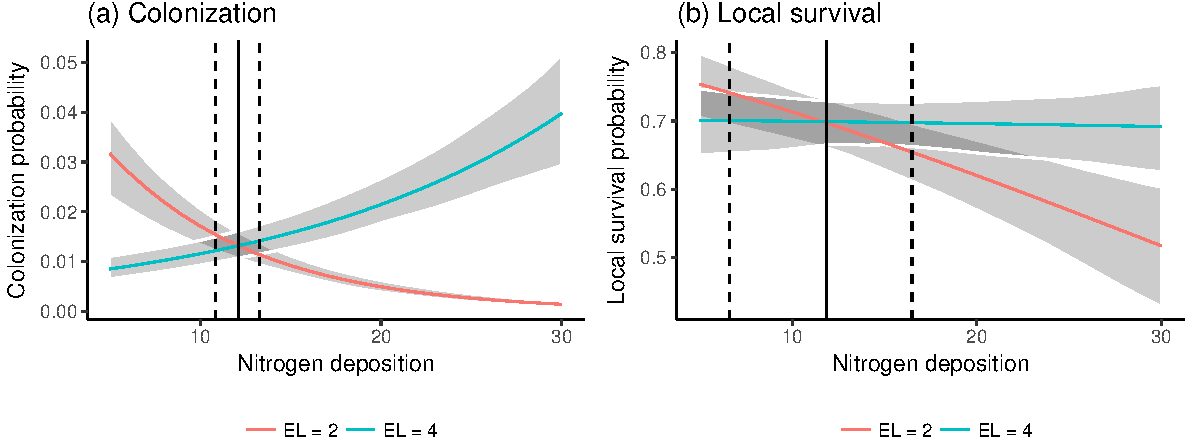
\includegraphics[width=1\linewidth]{Manuscript_files/figure-latex/neff-1} \caption{Colonization (a) and local survival (b) of oligotrophic (Ellenberg N = 2; red line) and eutrophic (Ellengerg N = 4) species along the N deposition gradient. Given are means and 95\%-Credible Intervals from logistic linear mixed models.}\label{fig:neff}
\end{figure}

\section*{Discussion}\label{discussion}
\addcontentsline{toc}{section}{Discussion}

\begin{itemize}
\item
  Any empty space that could be caused by any disturbance that let to
  the local disappearance of species is likely to be fiellied by
  eutrophic species. Disturbance depends on the site, while colonization
  depends on species characteristics.
\item
  The rather large spatial turnover might be partly explained by species
  that remained undetected in one of the surveys, but it might also be
  the result of species that newly colonized sites (species gains) and
  species that truely disappeared from sites (species losses).
\item
  Altough N deposition considerabely declinded between 2005 and 2015, we
  could not detect major shifts in plant community structure during the
  same time period.
\item
  Eutrophic species have rather high local survival across the entire
  deposition gradient, while oligotrophic species have much reduced
  local survival at high N deposition. This suggests that it takes much
  more time to replace eutrophic by oligotrophic species than replacing
  oligotrophic by eutrophic species.
\item
  Our data on colonization and local survival (i.e.~temporal variation)
  confirm the empirical critical loads that we infered from anlysing
  spatial co-variation of N deposition and species richness.
\item
  Local survival is higher for low temperature plants --\textgreater{}
  This could explain the decrease in cumminity change along elevation.
  This could also explain the differences at mount summets were space
  was empty in the beginning.
\item
  Climatic effects are more likely to be reversed thant effects due to
  fertilization.
\end{itemize}

\subsubsection{Space for time
substitution}\label{space-for-time-substitution}

Often observational studies infer the change of plant diversity along a
gradient of N deposi- tion. Thus, they infer how the spatial variation
in species richness is related to N deposition and assume that this
spatial variation in species richness arose because over time some areas
lost more species than others because they chronically experienced
higher N deposition. Alt- hough there is evidence supporting the use of
such a `space for time substitution' for detecting the effects of N
deposition on plant diversity (Stevens et al. 2010), they can not
replace stud- ies that relate temporal patterns in species with N
deposition (De Schrijver et al. 2011). While recovery of acidified
surface waters has been well investigated (De Vries et al. 2015), there
are only a limited number of studies inferring temporal trends of plant
species diversity relat- ed to varying amounts of N-deposition. Storkey
et al. (2015) demonstrated a positive response of biodiversity to
reducing N addition from either atmospheric pollution or fertilizers in
the Park Grass Experiment: «The proportion of legumes, species richness
and diversity increased across the experiment between 1991 and 2012 as
N-deposition declined». For forest floor vegetation in permanent plots
across Europe the exceedance of critical loads of N over a peri- od from
9 to 42 years had negative effects on the cover of oligotrophic plant
species, i.e spe- cies that prefer nutrient-poor soils, although species
richness remained constant (Dirnböck et al. 2014). Another example of
recovery in eutrophicated habitats gives the recovery of species
richness in previously fertilized plots (Clark and Tilman 2008). In this
study, the recorded recovery in species richness within one or two
decade was likely due to the species rich vege- tation surrounding the
experimental plots, from where immigration was easily feasible.

\begin{quote}
Hier sagen, dass der CRL identisch wie der CRL von räumlichen
Zusammenhängen ist.
\end{quote}

\section*{Conclusions}\label{conclusions}
\addcontentsline{toc}{section}{Conclusions}

xxx

\section*{Acknowledgements}\label{acknowledgements}
\addcontentsline{toc}{section}{Acknowledgements}

We thank the dedicated and qualified botanists who conducted fieldwork.
The Swiss Federal Office for the Environment (FOEN) kindly provided
biodiversity monitoring data and topographic data. This work was
supported by the FOEN, the Swiss National Science Foundation (grant no.
31003A\_156294), the Swiss Association Pro Petite Camargue Alsacienne,
the Fondation de bienfaisance Jeanne Lovioz, and the MAVA Foundation.

\section*{References}\label{references}
\addcontentsline{toc}{section}{References}

\hypertarget{refs}{}
\hypertarget{ref-Hillebrand2018}{}
Hillebrand, Helmut, Bernd Blasius, Elizabeth T. Borer, Jonathan M.
Chase, John A. Downing, Britas Klemens Eriksson, Christopher T.
Filstrup, et al. 2018. ``Biodiversity Change Is Uncoupled from Species
Richness Trends: Consequences for Conservation and Monitoring.''
\emph{Journal of Applied Ecology} 55 (1): 169--84.
doi:\href{https://doi.org/10.1111/1365-2664.12959}{10.1111/1365-2664.12959}.



\end{document}
